\begin{frame}[fragile]
	\frametitle{Vordefinierte Zähler}
	
	\begin{center}
		\begin{tabular}{ll}
			\emphword{Dokument} & \keyword{page} \\[0.5cm]
			\emphword{Kapitel} & \keyword{part}, \keyword{chapter}, \keyword{section}, \keyword{subsection}, \keyword{subsubsection} \\
			& \keyword{paragraph}, \keyword{subparagraph} \\[0.5cm]
			\emphword{Aufzählung} & \keyword{enumi}, \keyword{enumii}, \keyword{enumiii}, \keyword{enumiv} \\[0.5cm]
			\emphword{Umgebungen} & \keyword{equation}, \keyword{figure}, \keyword{table}, \keyword{footnote}
		\end{tabular}
	\end{center}
\end{frame}

\begin{frame}[fragile]
	\frametitle{Eigene Längen}
	
	\begin{center}
		\begin{tabular}{ll}
			\befehl{newlength\{}\befehl{laenge\}} & neue Längenvariable anlegen \\
			\befehl{setlength\{}\befehl{laenge\}\{x\}} & Länge auf \keyword{x} setzen \\
			\befehl{addtolength\{}\befehl{laenge\}\{x\}} & Länge um \keyword{x} erhöhen\\
			\befehl{settolength\{}\befehl{laenge\}\{text\}} & Länge von \keyword{text} speichern\\
			\befehl{settoheight\{}\befehl{laenge\}\{text\}} & Höhe von \keyword{text} speichern \\
			\befehl{settodepth\{}\befehl{laenge\}\{text\}} & Größter Abstand zur Basislinie
		\end{tabular}
	\end{center}
\end{frame}

\begin{frame}[fragile]
	\frametitle{Vordefinierte Längen}
		\begin{columns}[T]
		\begin{column}{0.54\textwidth} \vspace{-1cm}
			\begin{enumerate}
				\item \befehl{hoffset}
				\item \befehl{voffset}
				\item \befehl{oddsidemargin}
				\item \befehl{topmargin}
				\item \befehl{headheight}
				\item \befehl{headsep}
				\item \befehl{textheight}
				\item \befehl{textwidth}
				\item \befehl{marginparsep}
				\item \befehl{marginparwidth}
				\item \befehl{marginpar}
				\item \befehl{footskip}
				\item[~] \befehl{paperwidth}, \befehl{paperheight}
			\end{enumerate}
		\end{column}
		\begin{column}{0.44\textwidth} \vspace{-3cm}
			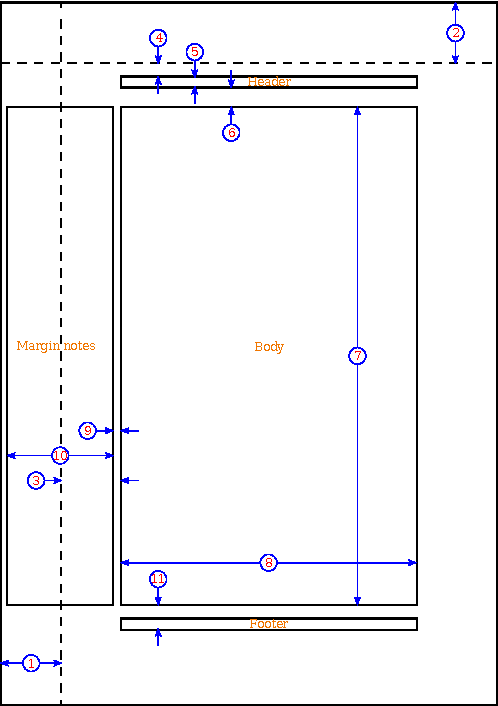
\includegraphics[scale=1.2]{img/page_layout.pdf}
		\end{column}
	\end{columns}
\end{frame}
